
%================================================
\begin{frame}[fragile]{Language Expressivity}
    \begin{itemize}
        \item Function definition and composition
        \item Anonymity
        \item Faust programs as components
        \item Libraries, namespaces
        \item Partial application
        \item Lexical environments as first class citizen
        \item Pattern Matching (meta programmation = algorithmic description of circuits)
    \end{itemize}
\end{frame}


\begin{frame}[fragile,shrink=30]{Language Expressiveness}{Fast Fourier Transform}
    \vspace{1cm}
    \begin{lstlisting}
    fft(N) = si.cbus(N) : an.c_bit_reverse_shuffle(N) : fftb(N)
    with {
        fftb(1) = _,_;
        fftb(N) = si.cbus(N)
                : (fftb(No2)<:(si.cbus(No2), si.cbus(No2))),
                (fftb(No2) <: (si.cbus(N):twiddleOdd(N)))
                :> si.cbus(N)
            with {
            No2 = int(N)>>1;
            twiddleOdd(N) = par(k,N,si.cmul(cos(w(k)),0-sin(w(k))));
            w(k) = 2.0*ma.PI*float(k)/float(N);
            };
    };
    
    \end{lstlisting}
\end{frame}
        
\begin{frame}[fragile,shrink=30]{Language Expressiveness}{Fast Fourier Transform}
    \vspace{1cm}
    \begin{lstlisting}
        fft(1)
    \end{lstlisting}

    \begin{center}
        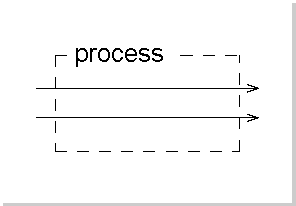
\includegraphics[width=1\textwidth]{images/fft1}
    \end{center}
\end{frame}
 
    
\begin{frame}[fragile,shrink=30]{Language Expressiveness}{Fast Fourier Transform}
    \vspace{1cm}
    \begin{lstlisting}
        fft(2)
    \end{lstlisting}

    \begin{center}
        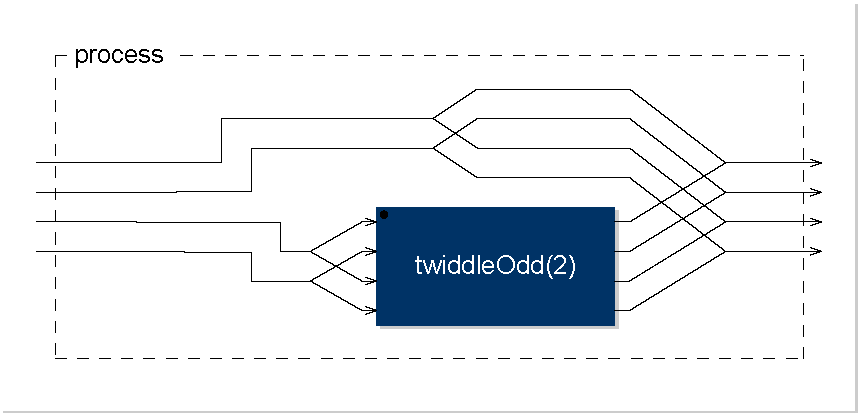
\includegraphics[width=1\textwidth]{images/fft2}
    \end{center}
\end{frame}
    
\begin{frame}[fragile,shrink=30]{Language Expressiveness}{Fast Fourier Transform}
    \vspace{1cm}
    \begin{lstlisting}
        fft(4)
    \end{lstlisting}

    \begin{center}
        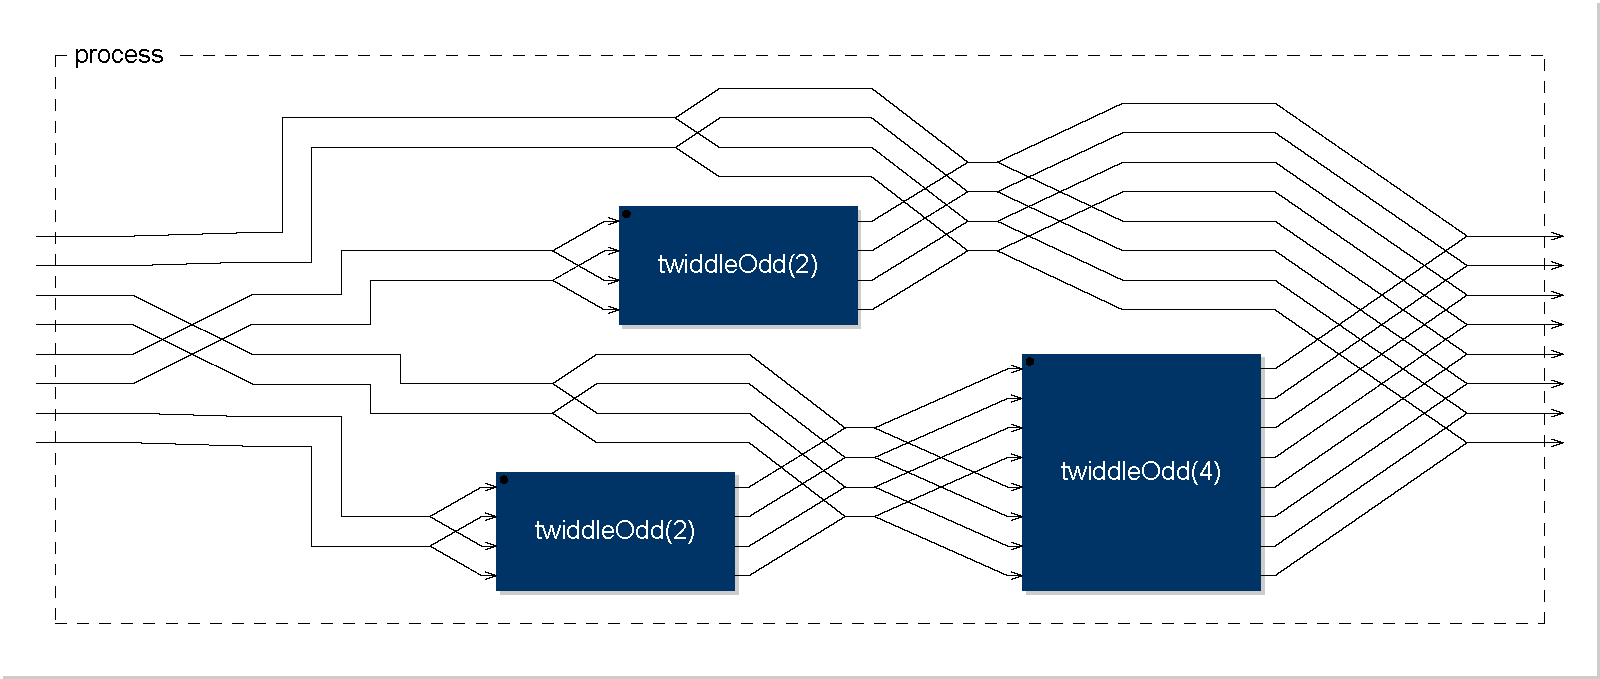
\includegraphics[width=1\textwidth]{images/fft4}
    \end{center}
\end{frame}
    
\begin{frame}[fragile,shrink=30]{Language Expressiveness}{Fast Fourier Transform}
    \vspace{1cm}
    \begin{lstlisting}
        fft(8)
    \end{lstlisting}

    \begin{center}
        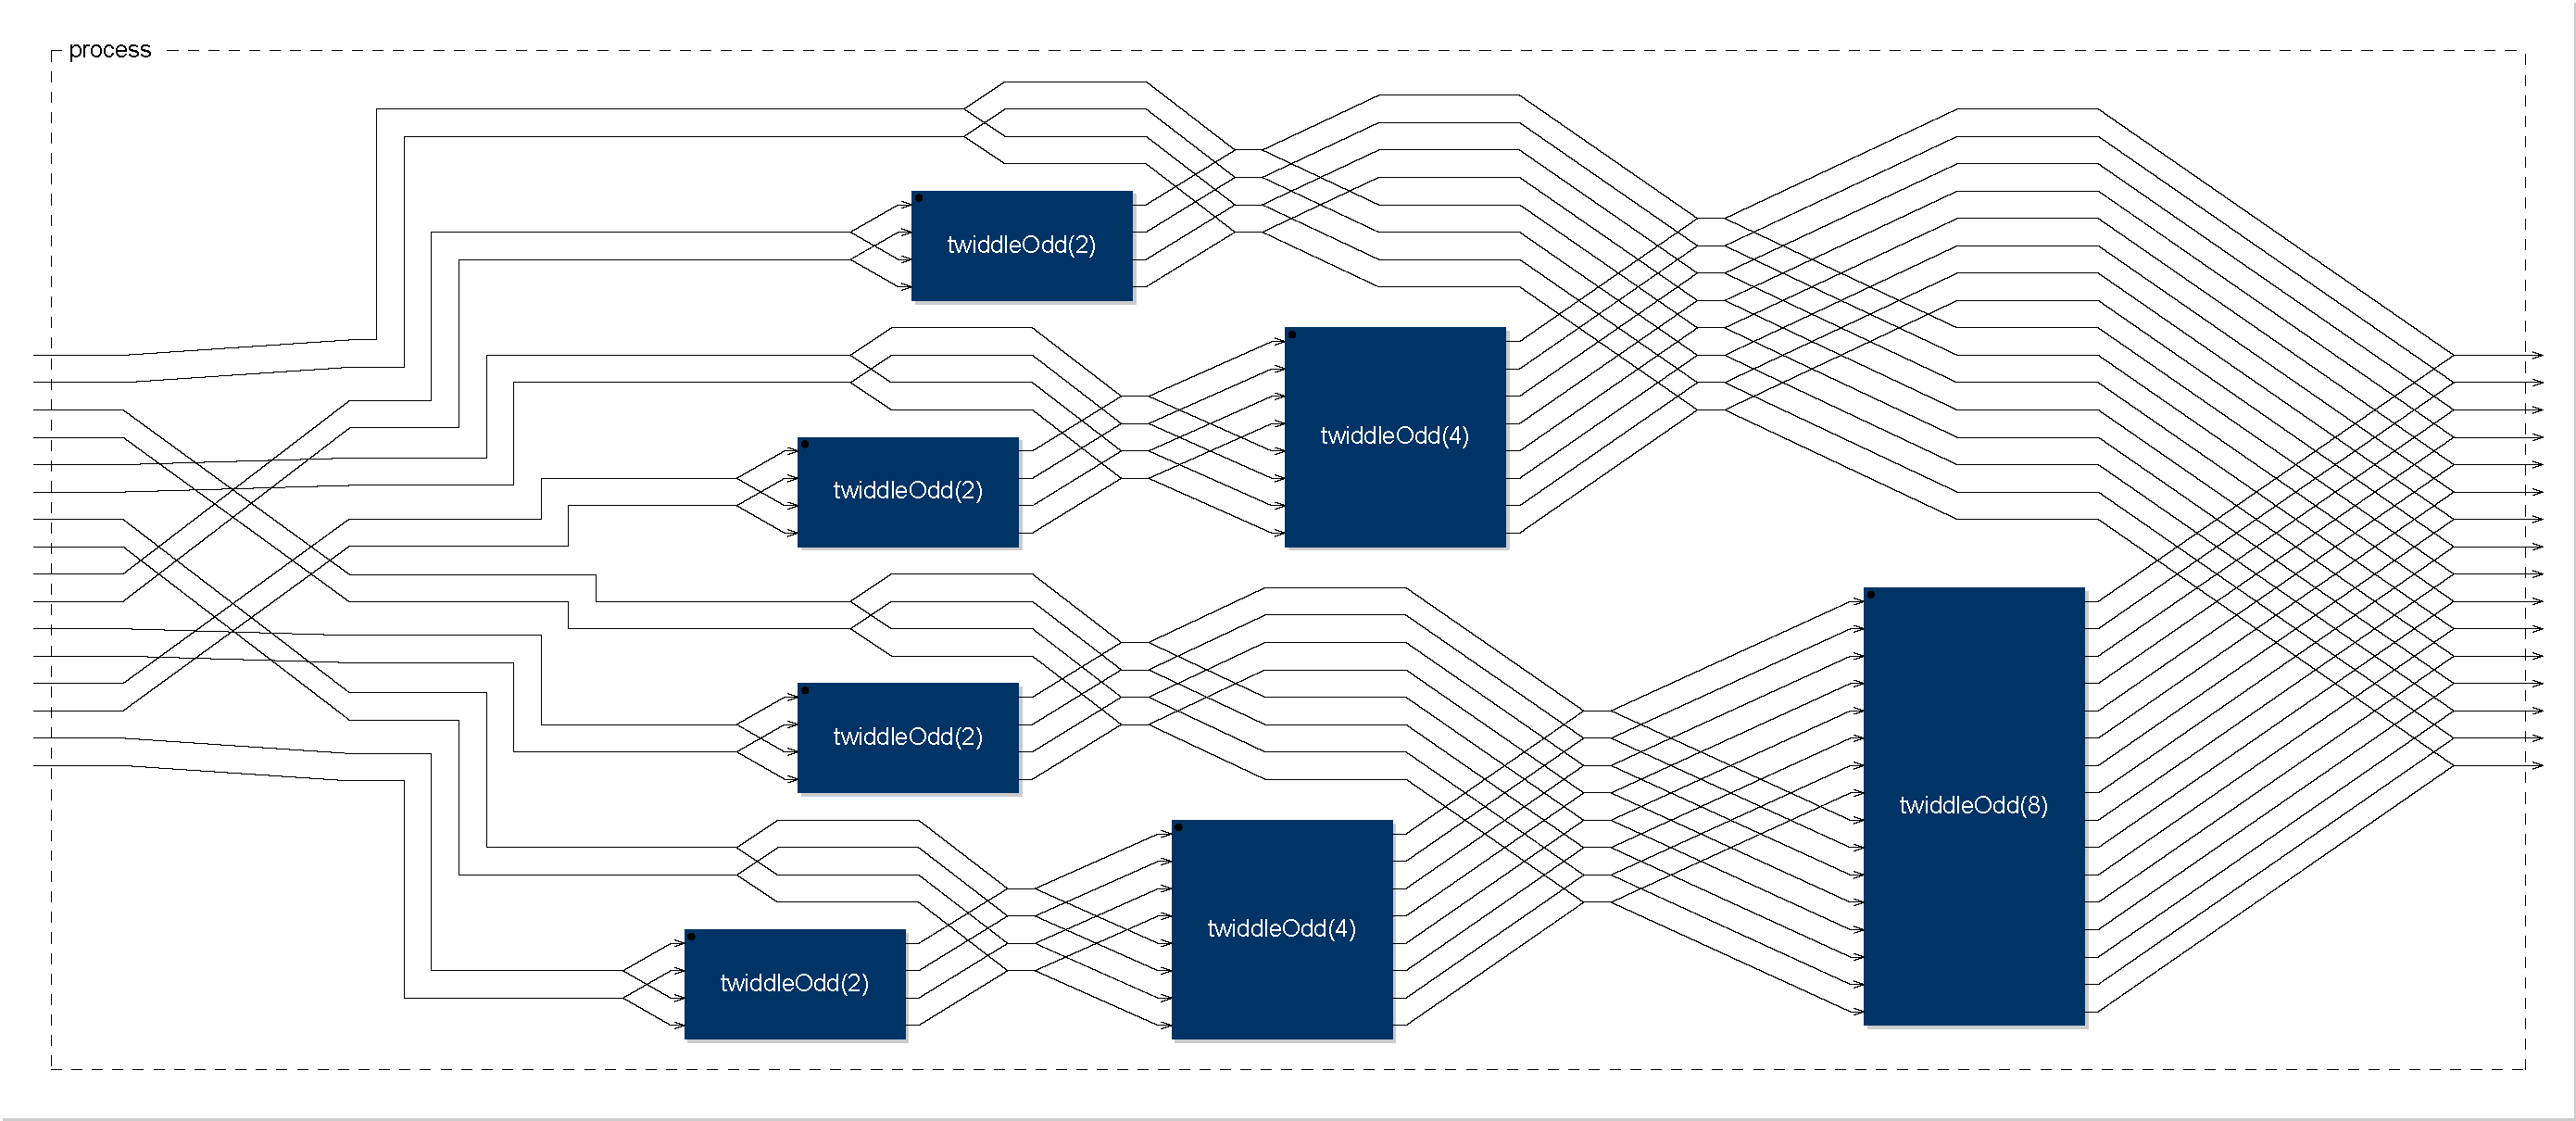
\includegraphics[width=1\textwidth]{images/fft8}
    \end{center}
\end{frame}
    
\begin{frame}[fragile,shrink=30]{Language Expressiveness}{Fast Fourier Transform}
    \vspace{1cm}
    \begin{lstlisting}
        fft(16)
    \end{lstlisting}

    \begin{center}
        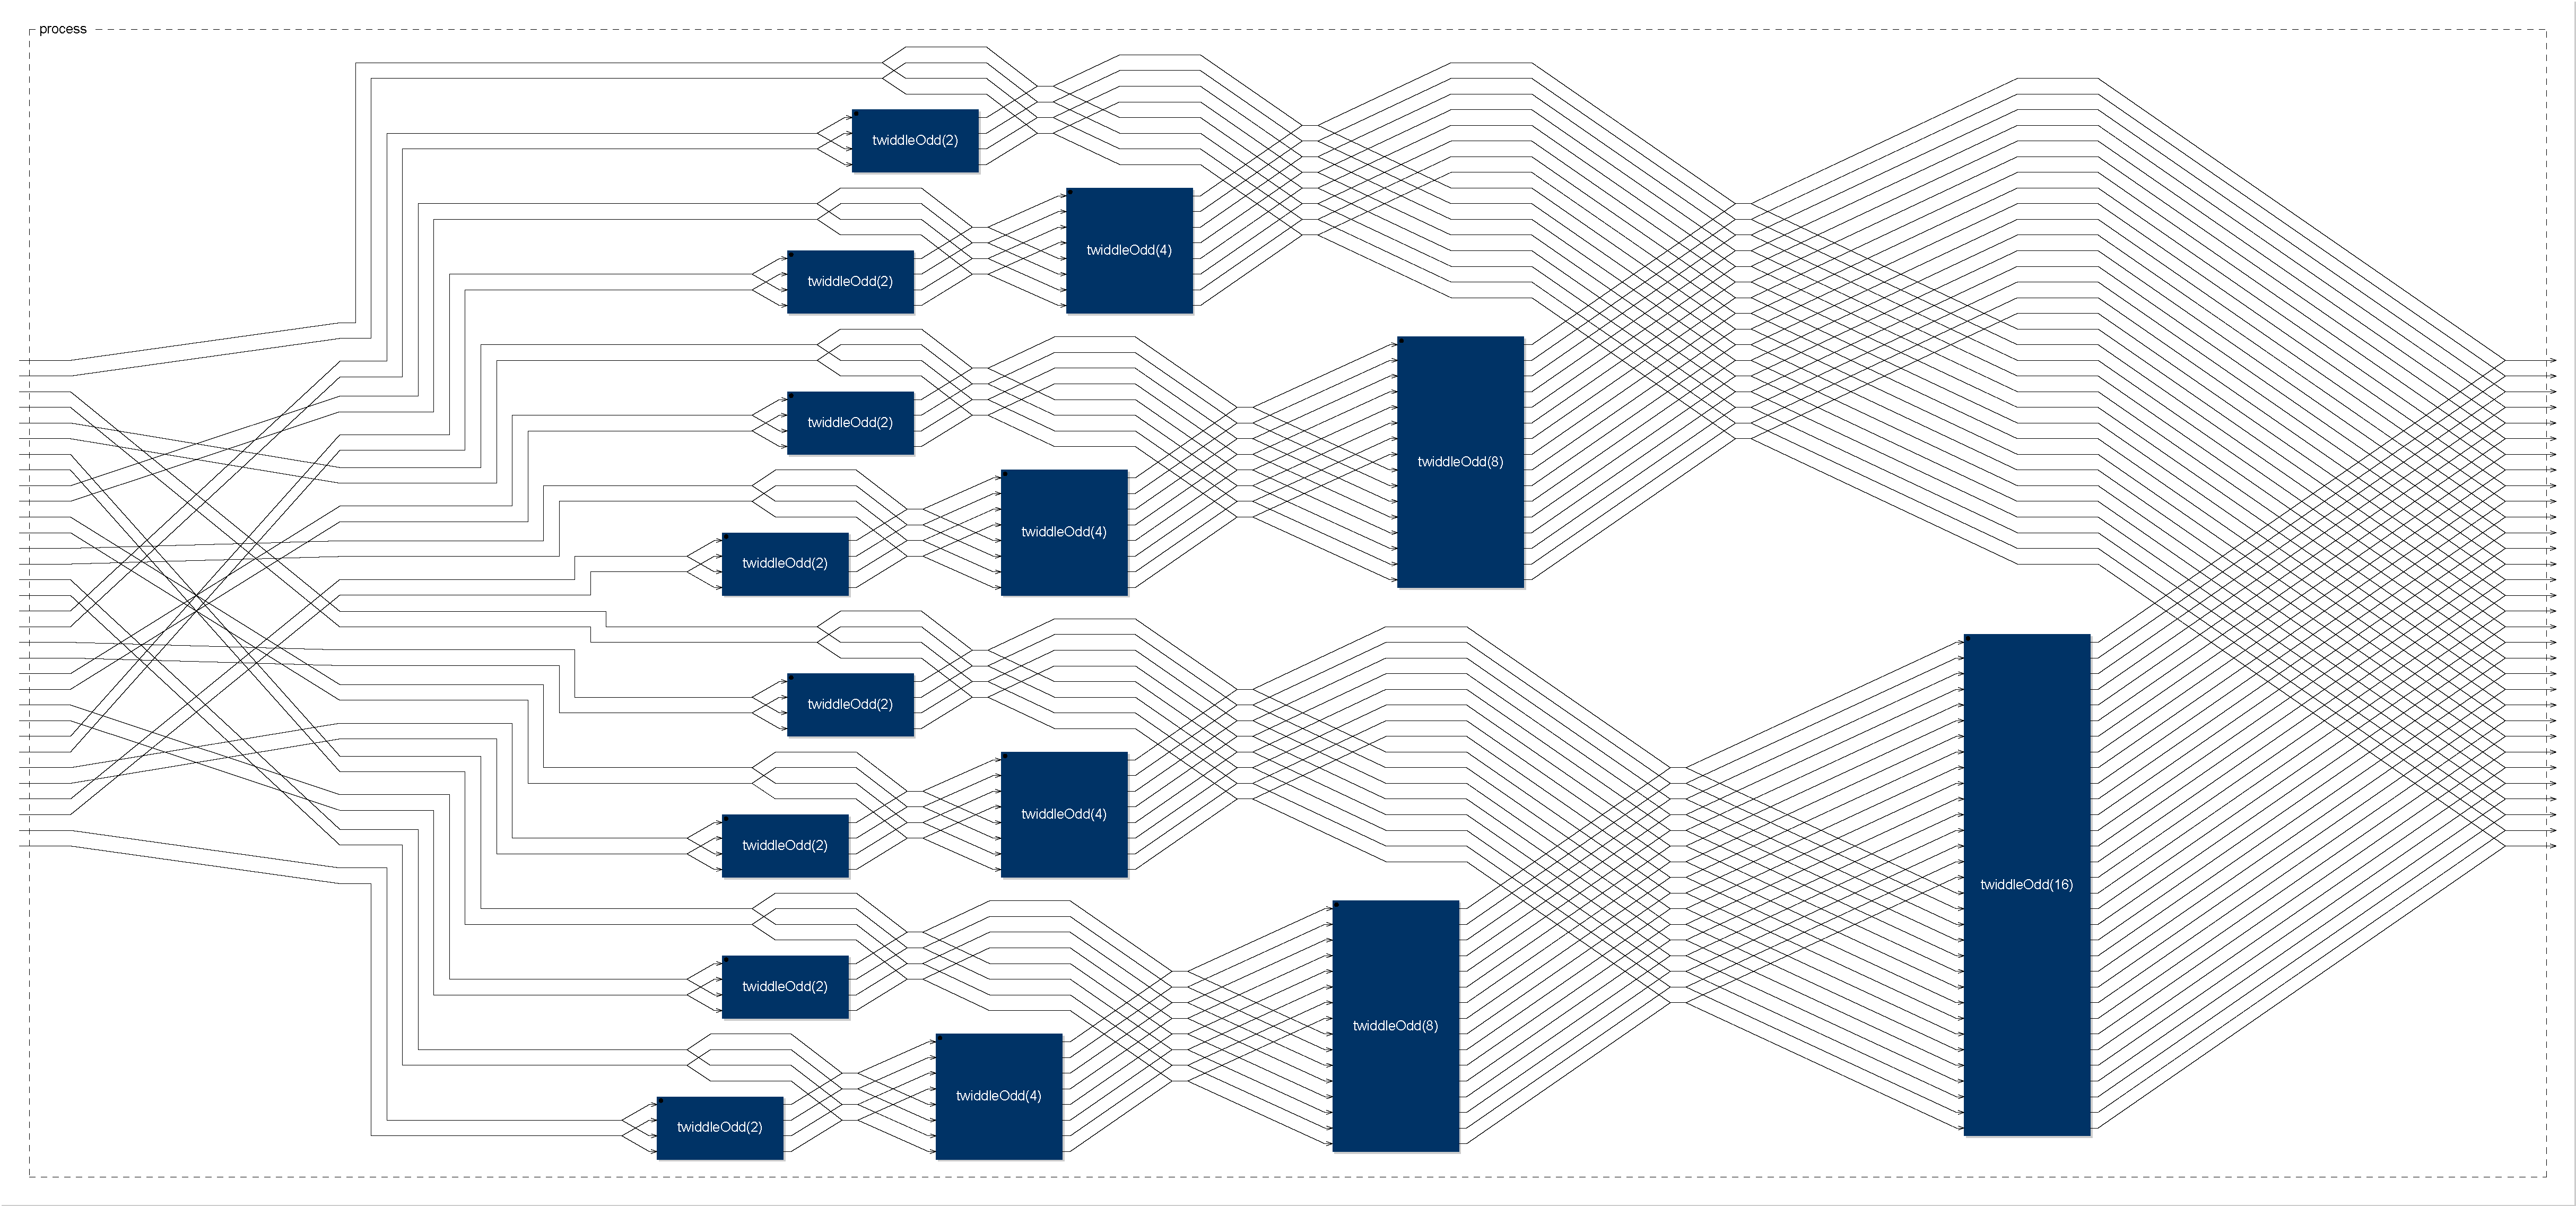
\includegraphics[width=1\textwidth]{images/fft16}
    \end{center}
\end{frame}
    
\begin{frame}[fragile,shrink=30]{Language Expressiveness}{Fast Fourier Transform}
    \vspace{1cm}
    \begin{lstlisting}
        fft(32)
    \end{lstlisting}

    \begin{center}
        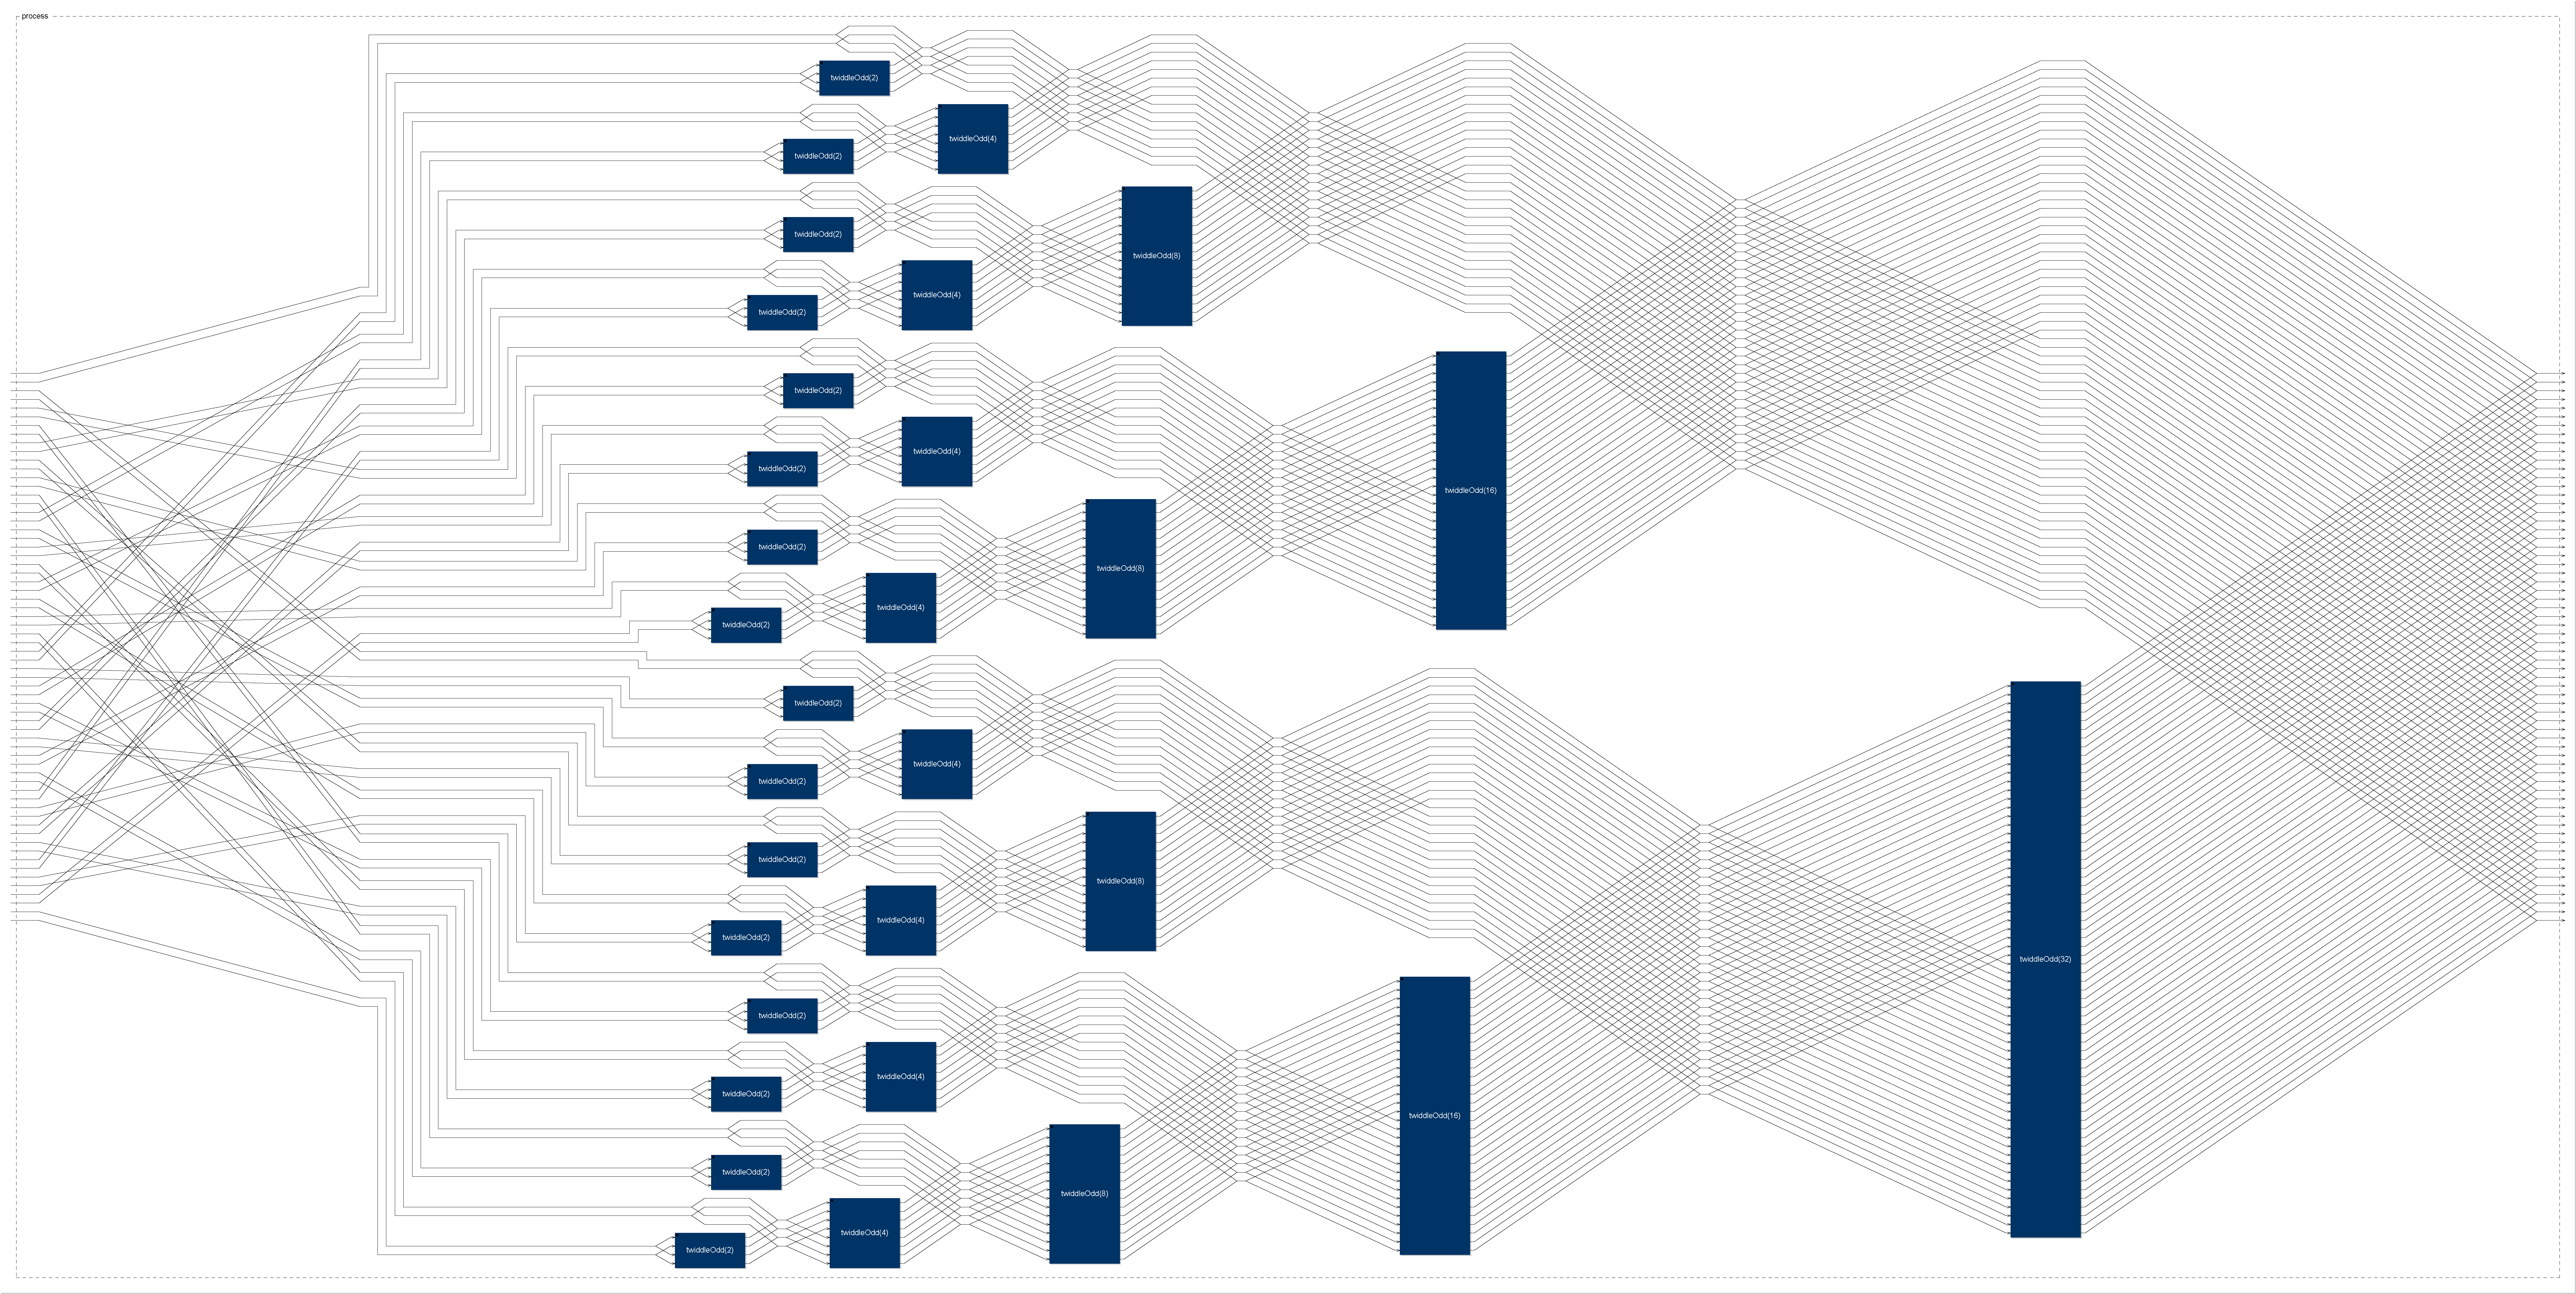
\includegraphics[width=1\textwidth]{images/fft32}
    \end{center}
\end{frame}
    
\begin{frame}[fragile,shrink=30]{Language Expressiveness}{Fast Fourier Transform}
    \vspace{1cm}
    \begin{lstlisting}
        fft(64)
    \end{lstlisting}

    \begin{center}
        \includegraphics[width=1\textwidth]{images/fft64}
    \end{center}
\end{frame}

